% ! TeX root = ./document.tex
\documentclass[9pt, aspectratio=169, handout]{beamer}
% ! TeX root = ../document.tex
\usepackage[utf8]{inputenc}
\usepackage{multicol}
\usepackage{pgfpages}
\usepackage{roboto}
\usepackage{PlayfairDisplay}
\usepackage{fontawesome5}
\usepackage[T1]{fontenc}
\usepackage[final]{pdfcomment}
\usepackage{minted}
\usepackage[backend=bibtex,style=alphabetic,sorting=none,doi=true,url=false]{biblatex} 
\usepackage{xargs}
% ! TeX root = ../document.tex
\usetheme{material}
\useDarkTheme
\usePrimaryRed
\useAccentGreen

% ! TeX root = ../document.tex

\title{
  {\fontfamily{\playfairfamily}\fontseries{black}\selectfont
    Towards Reinforcement Learning-based \\ Aggregate Computing
  }
}
\author[G.Aguzzi]{
  \textbf{Gianluca Aguzzi}\inst{1}, Roberto Casadei \inst{1}, Mirko Viroli \inst{1}
}
\institute{
  \inst{1}
  \texttt{Alma Mater Studiorum} -- Università di Bologna, Cesena, Italy
}
\talk{
  Talk @ COORDINATION 2022
}

\bibliography{biblio.bib}
\begin{document}
\begin{frame}[plain]
\titlepage
\end{frame}

\section{Background}
\begin{frame}{Background}
  \begin{card}[Computing Systems of \textbf{Tomorrow} (Today?)]
    \begin{itemize}
      \item \highlight{Smart} things ``everywhere'' (\emph{pervasive}, \emph{ubiquitous}, \emph{collective} computing)
      \item Dense, layered and complex large scale IT networks (\emph{cloud-fog-edge} computing)
      \item \highlight{Opportunistic} and \highlight{situated}-aware computing
    \end{itemize}
  \end{card}
  \begin{alarm}[Challenges]
    \begin{itemize}
      \item \highlight{Collective} \& \highlight{self-adaptive} behaviours \emph{\faArrowRight} Collective Adaptive Systems (CASs)
      \begin{itemize}
        \item \highlight{coordination}: how entities interact to reach collective goal?
        \item \highlight{self-organization}: how to mantain a system in order?
      \end{itemize}
      \item Distributed control, local-to-global problem, openness, \dots
      \item \emph{How} can we program such kind of systems?
    \end{itemize}
  \end{alarm}
\end{frame}

\begin{frame}{Aggregate Computing}
  \begin{cardTiny}
    \begin{itemize}
      \item <1-> A top-down global-to-local macro-programming approach to express \highlight{collective} \& \highlight{self-organising} behaviour
      \item <2-> \highlight{Computational field} as a first-class abstraction for expressing system dynamics
      \begin{itemize}
        \item Computational field is a macro-abstraction that maps a set of devices over time to computational values
        \item [\success{\faThumbsUp}] \highlight{Functional appraoch}: distributed program expressed as a functional application through computational fields
      \end{itemize}
    \end{itemize}
  \end{cardTiny}
  \begin{multicols}{2}
    \begin{card}[Benefits]
      \begin{itemize}
        \item Programs expressed thinking about macro-properties
        \item \highlight{Scale-independent} \& \highlight{self-stabilising} collective behaviours
      \end{itemize}
    \end{card}
    \begin{cardTiny}
      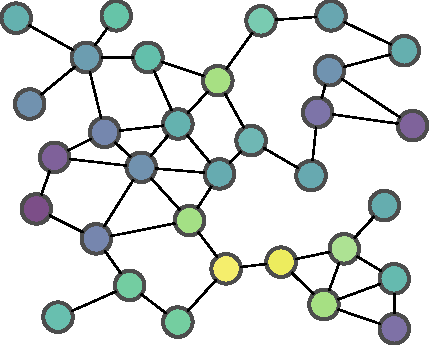
\includegraphics[width=0.45\textwidth]{img/discrete.pdf}
      \hfill
      %\parbox[c]{0.1\textwidth}{\Large  \vspace*{\fill} \strut \faArrowRight \vspace*{\fill}}
      \parbox[c]{1em}{\color{primary}\vspace*{-6em}\Large \faArrowRight}
      \hfill
      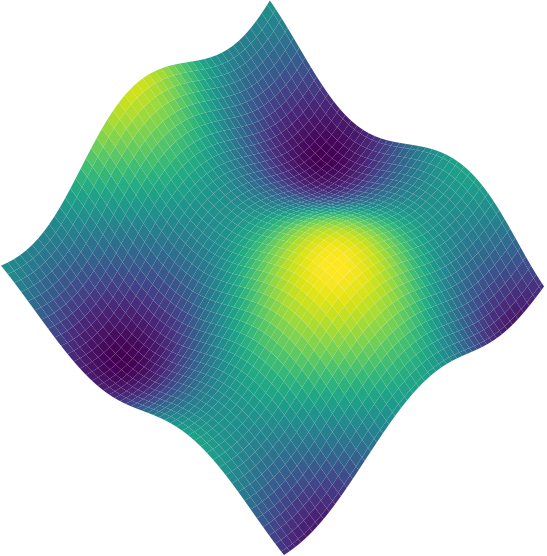
\includegraphics[width=0.38\textwidth]{img/viridis-result.png}
    \end{cardTiny}
  \end{multicols}
\end{frame}
\begin{frame}[fragile]{Aggregate Computing -- In a nutshell}
  \begin{multicols}{2}
    \begin{card}[Gradient]
    \begin{minted}{scala}
val gradient = rep(Inf)(distance =>
mux(isCenter){0.0}/*else*/{
  includingSelf.
    minHood(nbr{distance} + nbrRange)
})
    \end{minted}
    \end{card}
    \begin{card}[Distributed sensing]
    \begin{minted}{scala}
val leader = S(radius)
val potential = distanceTo(leader)
val mean =
  collectMean(potential, temperature)
broadcast(leader, mean)
  \end{minted}  
  \end{card}
    
  \end{multicols}
\end{frame}
\section{Conclusion}
\begin{frame}{Conclusion}

\end{frame}


\begin{frame}[allowframebreaks]
  \frametitle{References}
  \printbibliography
\end{frame}
\end{document}
